\documentclass[a4paper,12pt]{report}
\usepackage[slovene]{babel}
\usepackage{listings}
\usepackage{graphicx}
\usepackage[section]{placeins}

\lstset{
numberstyle=\small, 
numbersep=8pt, 
frame = single, 
language=SQL, 
framexleftmargin=15pt}

\begin{document}

\title{TUP: 2. in 3. domača naloga}
\author{Jakob Marušič}
\maketitle

\chapter*{2. domača naloga: Pretvorba konceptualnega modela v relacije}

\section*{Obrazložitev}
V nadaljevanju pošiljam rešitve 2. domače naloge. Rok za oddajo sem namreč po neumnosti zamudil, vendar pa bi vseeno želel, da se lahko pri popravljanju tretje domače naloge nanašate na kontekst 2.
\pagebreak

\section*{Naloga (a)}

\paragraph{Navodila}
\begin{em}
  V relacije preslikajte s pomočjo orodja Power Designer (Generate physical model), kjer iz slike dobljenega logičnega modela prepišete strukturo relacij, npr. Relacija(A, B, \#C).
\end{em}


\begin{center}
  \begin{tabular}{ ||p{15cm}|| }
    \hline
    Relacije \\
    \hline \hline
    kraj(\underline{postna\_stevilka}, kraj)\\ \\
    naslov(\underline{naslovID}, \#postna\_stevilka, ulica, hisna\_stevilka)\\ \\
    pacient(\underline{stevilka\_KZZ}, \#naslovID, ime, priimek, rojstni\_datum, spol)\\ \\
    diagnoza\_pacient(\underline{\#stevilka\_KZZ, \#id\_diagnoze}, stevilka\_diagnoze)\\ \\
    diagnoza(\underline{id\_diagnoze}, slovenska\_kvalifikacija, angleska\_kvalifikacija, mednarodna\_kvalifikacija)\\ \\
    obravnava(\underline{stevilka\_obravnave}, \#stevilka\_obravnave)\\ \\
    cakalna\_vrsta(\underline{\#stevilka\_obravnave, \#stevilka\_oddelka}, datum\_vpisa, cas\_vpisa, predviden\_datum\_sprejema, predviden\_cas\_sprejema)\\
    oddelek(\underline{stevilka\_oddelka}, ime\_oddelka)\\ \\
    izvid\_preiskave(\underline{stevilka\_preiskave}, \#id\_samoplacnika, \#sifra\_preiskave, \#stevilka\_obravnave, datum\_šreiskave, cas\_preiskave, rezultat\_preiskave)\\
    samoplacnik(\underline{id\_samoplacnika})\\ \\
    preiskava(\underline{sifra\_preiskave}, ime preiskave, min\_dopustni\_interval, max\_dopustni\_interval, cena\_za\_samoplacnike)\\ \\
    referencna\_vrednost\_moski(\underline{sifra\_preiskave}, ime\_preiskave, min\_dopustni\_interval, max\_dopustni\_interval, cena\_za\_samoplacnike, min\_referencna\_vrednost, max\_referencna\_vrednost)\\ \\
    referencna\_vrednost\_zenske(\underline{sifra\_preiskave}, ime\_preiskave, min\_dopustni\_interval, max\_dopustni\_interval, cena\_za\_samoplacnike, min\_referencna\_vrednost, max\_referencna\_vrednost)\\ \\
    \hline
  \end{tabular}
\end{center}

\section*{Naloga (b)}
\paragraph{Navodila}
\begin{em}
  V relacije preslikajte ročno, po navodilih in priporočilih s predavanj.
\end{em}

\paragraph{}
  \begin{center}
    \begin{tabular}{ ||p{15cm}|| }
      \hline
      Relacije \\
      \hline \hline
      kraj(\underline{postna\_stevilka}, kraj)\\ \\
      naslov(\underline{naslovID}, \#postna\_stevilka, ulica, hisna\_stevilka)\\ \\
      pacient(\underline{stevilka\_KZZ}, \#naslovID, ime, priimek, rojstni\_datum, spol)\\ \\
      diagnoza\_pacient(\underline{\#stevilka\_KZZ, \#id\_diagnoze}, stevilka\_diagnoze)\\ \\
      diagnoza(\underline{id\_diagnoze}, slovenska\_kvalifikacija, angleska\_kvalifikacija, mednarodna\_kvalifikacija)\\ \\
      obravnava(\underline{stevilka\_obravnave}, \#stevilka\_obravnave)\\ \\
      cakalna\_vrsta(\underline{\#stevilka\_obravnave, \#stevilka\_oddelka}, datum\_vpisa, cas\_vpisa, predviden\_datum\_sprejema, predviden\_cas\_sprejema)\\
      oddelek(\underline{stevilka\_oddelka}, ime\_oddelka)\\ \\
      izvid\_preiskave(\underline{stevilka\_preiskave}, \#id\_samoplacnika, \#sifra\_preiskave, \#stevilka\_obravnave, datum\_šreiskave, cas\_preiskave, rezultat\_preiskave)\\
      samoplacnik(\underline{id\_samoplacnika})\\ \\
      preiskava(\underline{sifra\_preiskave}, ime preiskave, min\_dopustni\_interval, max\_dopustni\_interval, cena\_za\_samoplacnike, min\_referencna\_vrednost\_moski, max\_referencna\_vrednost\_moski, min\_referencna\_vrednost\_zenska, max\_referencna\_vrednost\_zenska)\\ \\
      \hline
  \end{tabular}
\end{center}

\pagebreak

\section*{Naloga (c)}
\paragraph{Navodila}
\begin{em}
  Primerjajte dobljeni množici relacij, naštejte razlike in jih poskušajte razložiti (po možnosti tudi odpraviti s spremembami v gradnikih konceptualnega modela).
\end{em}

\paragraph{}
Edina razlika se pojavi pri pretvorbi hierhije iz konceptnega model v logični. Pri ročni pretvorbi sem se odločil za združevanje entitetnih tipov, medtem, ko je avtomatska pretvorba v PowerDesigner-ju ohranila vse tri tabele, akr povzroči redundanco v tabelah \textit{referencna\_vrednost\_moski} in \textit{referencna\_vrednost\_zenska}.

\paragraph{}
Ker pri preslikavi hierhije ne obstaja določen postopek, vendar jih je več, se konceptnega modela (razen, da bi hierhijo popolnoma odstranili) ne da spremeniti do tega, da bi logična modela bila enaka.


\section*{Naloga (d)}
\paragraph{Navodila}
\begin{em}
  Dobljene relacije z orodjem PowerDesigner pretvorite v SQL skripto (za MySQL), kreirajte tabele in jih napolnite (lahko avtomatsko).
\end{em}

\paragraph{}\mbox{}
\begin{lstlisting}[language=SQL]
   create table diagnoza
   (  "id diagnoze"        int not null,
      "slovenska kvalifikacija" varchar(50),
      "angleska kvalifikacija" varchar(50),
      "mednarodna kvalifikacija" varchar(50),
      primary key ("id diagnoze")
   );
   create table "diagnoza pacient"
   (
      "stevilka KZZ"       int not null,
      "id diagnoze"        int not null,
      "stevilka diagnoze"  int not null,
      primary key ("stevilka KZZ", "id diagnoze")
   );
   create table "izvid preiskave"
   (
      "datum preiskave"    date,
      "cas preiskave"      time,
      "rezultat preiskave" float(5),
      "stevilka izvida"    int not null,
      "id samoplacnika"    int,
      "sifra preiskave"    int not null,
      "stevilka obravnave" int,
      primary key ("stevilka izvida")
   );
   create table kraj
   (
      "postna stevilka"    int not null,
      kraj                 varchar(20),
      primary key ("postna stevilka")
   );
   create table naslov
   (
      naslovID             int not null,
      "postna stevilka"    int not null,
      ulica                varchar(20),
      "hisna stevilka"     varchar(5),
      primary key (naslovID)
   );
   create table obravnava
   (
      "stevilka obravnave" int not null,
      "stevilka KZZ"       int not null,
      primary key ("stevilka obravnave")
   );
   create table oddelek
   (
      "stevilka oddelka"   int not null,
      "ime oddelka"        varchar(50),
      primary key ("stevilka oddelka")
   );
   create table pacient
   (
      "stevilka KZZ"       int not null,
      naslovID             int not null,
      ime                  varchar(20),
      priimek              varchar(50),
      "rojstni datum"      date,
      spol                 char(1),
      primary key ("stevilka KZZ")
   );
   create table preiskava
   (
      "sifra preiskave"    int not null,
      "ime preiskave"      varchar(20),
      "min dopustni interval" float(5),
      "max dopustni interval" float(5),
      "cena za samoplacnike" float(10),
      primary key ("sifra preiskave")
   );
   create table "referencna vrednost moski"
   (
      "sifra preiskave"    int not null,
      "ime preiskave"      varchar(20),
      "min dopustni interval" float(5),
      "max dopustni interval" float(5),
      "cena za samoplacnike" float(10),
      "min referencna vrednost" float(4),
      "max referencna vrednost" float(4),
      primary key ("sifra preiskave")
   );
   create table "referencna vrednost zenske"
   (
      "sifra preiskave"    int not null,
      "ime preiskave"      varchar(20),
      "min dopustni interval" float(5),
      "max dopustni interval" float(5),
      "cena za samoplacnike" float(10),
      "min referencni interval" float(4),
      "max referencni interval" float(4),
      primary key ("sifra preiskave")
   );
   create table samoplacnik
   (
      "id samoplacnika"    int not null,
      primary key ("id samoplacnika")
   );
   create table "cakalna vrsta"
   (
      "stevilka obravnave" int not null,
      "stevilka oddelka"   int not null,
      "datum vpisa"        date,
      "cas vpisa"          time,
      "predviden datum sprejema" date,
      "predviden cas sprejema" time,
      primary key 
      ("stevilka obravnave", "stevilka oddelka")
   );
   
   alter table "diagnoza pacient" 
      add constraint FK_ima 
      foreign key ("stevilka KZZ")
      references pacient ("stevilka KZZ") 
      on delete restrict on update restrict;
   
   alter table "diagnoza pacient" 
      add constraint "FK_je definirana z" 
      foreign key ("id diagnoze")
      references diagnoza ("id diagnoze") 
      on delete restrict on update restrict;
   
   alter table "izvid preiskave" 
      add constraint FK_definira 
      foreign key ("sifra preiskave")
      references preiskava ("sifra preiskave") 
      on delete restrict on update restrict;
   
   alter table "izvid preiskave" 
      add constraint "FK_pripada obravnavi" 
      foreign key ("stevilka obravnave")
      references obravnava ("stevilka obravnave") 
      on delete restrict on update restrict;
   
   alter table "izvid preiskave" 
      add constraint "FK_se prijavlja" 
      foreign key ("id samoplacnika")
      references samoplacnik ("id samoplacnika") 
      on delete restrict on update restrict;
   
   alter table naslov 
      add constraint "FK_se nahaja v" 
      foreign key ("postna stevilka")
      references kraj ("postna stevilka") 
      on delete restrict on update restrict;
   
   alter table obravnava 
      add constraint "FK_je obravnavan" 
      foreign key ("stevilka KZZ")
      references pacient ("stevilka KZZ") 
      on delete restrict on update restrict;
   
   alter table pacient 
      add constraint FK_pripada 
      foreign key (naslovID)
      references naslov (naslovID) 
      on delete restrict on update restrict;
   
   alter table "referencna vrednost moski" 
      add constraint FK_referenca 
      foreign key ("sifra preiskave")
      references preiskava ("sifra preiskave") 
      on delete restrict on update restrict;
   
   alter table "referencna vrednost zenske" 
      add constraint FK_referenca2 
      foreign key ("sifra preiskave")
      references preiskava ("sifra preiskave") 
      on delete restrict on update restrict;
   
   alter table "cakalna vrsta" 
      add constraint "FK_je umescen" 
      foreign key ("stevilka obravnave")
      references obravnava ("stevilka obravnave") 
      on delete restrict on update restrict;
   
   alter table "cakalna vrsta" 
      add constraint "FK_pripada oddelku" 
      foreign key ("stevilka oddelka")
      references oddelek ("stevilka oddelka") 
      on delete restrict on update restrict;
   
\end{lstlisting}

\section*{Naloga (e)}
\paragraph{Navodila}
\begin{em}
  Opišite pet (5) smiselnih netrivialnih operacij nad podanimi tabelami, ter jih implementirajte v obliki SQL poizvedb (vsaka nad najmanj dvema tabelama, vsaj 3 gnezdene ali agregatne poizvedbe).
\end{em}

\subsection*{Poizvedba 1}
\paragraph{Opis poizvedbe}
Poizvedba za vsakega izmed samoplačnikov v bazi izračuna skupno ceno izvedenih preiskav.

\paragraph{SQL poizvedba}\mbox{}\\
\begin{lstlisting}[language = SQL]
select
  id_samoplacnika,
  sum(cena_za_samoplacnika)
from izvid_preiskave
join preiskava p on 
  izvid_preiskave.sifra_preiskave = p.sifra_preiskave
group by id_samoplacnika;
\end{lstlisting}

\pagebreak
\subsection*{Poizvedba 2}
\paragraph{Opis poizvedbe}
Poizvedba prikaže osebne podatke vseh pacientov, ki so potrebni za pošiljanje izvidov po pošti.

\paragraph{SQL poizvedba}\mbox{}\\
\begin{lstlisting}[language = SQL]
select
    p.ime,
    p.priimek,
select
    p.ime,
    p.priimek,
    n.ulica,
    n.hisna_stevilka,
    n.postna_stevilka
from
    pacient p
inner join naslov n on
    p.naslovID = n.naslovID;
\end{lstlisting}

\subsection*{Poizvedba 3}
\paragraph{Opis poizvedbe}
Poizvedba prikaže število pacientov, ki so ovrščeni na čakalno listo oddelka. Oddelki so razvrščeni od oddelka z najdaljšo čakalno vrsto do oddelka z najkrajšo.

\paragraph{SQL poizvedba}\mbox{}\\
\begin{lstlisting}[language = SQL]
select
  o.ime_oddelka as 'Ime oddelka',
  count(c.stevilka_obravnave) as 'V cakalni vrsti'
from
   cakalna_vrsta c
inner join oddelek o on 
      c.stevilka_oddelka = o.stevilka_oddelka
group by c.stevilka_oddelka
order by count(c.stevilka_obravnave) DESC;
\end{lstlisting}


\subsection*{Poizvedba 4}
\paragraph{Opis poizvedbe}
Poizvedba za vsakega izmed obravnavanih pacientov prikaže število obravnav.

\paragraph{SQL poizvedba}\mbox{}\\
\begin{lstlisting}[language = SQL]
select
  p.stevilka_KZZ,
  count(o.stevilka_KZZ)
from pacient p
inner join obravnava o on 
      p.stevilka_KZZ = o.stevilka_KZZ
group by o.stevilka_KZZ;
\end{lstlisting}

\subsection*{Poizvedba 5}
\paragraph{Opis poizvedbe}
Poizvedba za izbranega pacienta izpiše seznam diagnoz s slovensko kvalifikacijo. Diagnoze so urejene po številki diagnoze.

\paragraph{SQL poizvedba}\mbox{}\\
\begin{lstlisting}[language = SQL]
select
  p.stevilka_KZZ,
  p.ime,
  p.priimek,
  dp.stevilka_diagnoze,
  d.slovenska_kvalifikacija
from diagnoza_pacient dp
inner join diagnoza d on dp.id_diagnoze = d.id_diagnoze
inner join pacient p on dp.stevilka_KZZ = p.stevilka_KZZ
where p.stevilka_KZZ = :izbrani_pacient;
\end{lstlisting}

\chapter*{3. domača naloga}

\section*{Naloga (a)}
\paragraph{Navodila}
Definirajte mehanizem, ki bo preprečeval, da bi pacientu v okviru ISTE obravnave ISTI test naredili več kot dvakrat.

\paragraph{}\mbox{}
\begin{lstlisting}[language = SQL]
   DELIMITER $$

   CREATE TRIGGER ista_obravnava
   BEFORE INSERT
   ON izvid
   BEGIN

      DECLARE @test int

      SELECT @retVal = COUNT(vrednost) 
      FROM izvid
      WHERE st_obravnave = :obravnava 
            AND ime_preiskave = :preiskava

      IF (@retVal < 2 ) THEN
      BEGIN
          --DOVOLIMO IN VSTAVIMO NOV IZVID
      END IF
   
   END $$

\end{lstlisting}

\section*{Naloga (b)}
\paragraph{Navodila}
Definirajte operacije (transakcije), ki jih je potrebno izvesti brez prekinjanja.
\textit{Baza avtomatsko preveri ali vnos novega podatka ne krši primarnih in tujih ključev. Predvideva se, da so vsi oddelki, vrste preiskav in kode diagnoz v bazi že vnešeni}

\paragraph{Dodajanje novega izvida 1}
V kolikor obravnava še ni odprta za danega pacienta moramo kot del transakcije izvesti:
\begin{enumerate}
   \item Pacientu dodamo novo obravnavo na danem oddelku
   \item Pacientu določimo nov izvid (rezultat preiskave)
\end{enumerate}

\paragraph{Dodajanje novega izvida 2}
V kolikor pacient v bazi še ne obstaja moramo kot transkacijo izvesti:
\begin{enumerate}
   \item V bazo dodamo pacienta
   \item Pacientu dodamo novo obravnavo na danem oddelku
   \item Pacientu določimo nov izvid (rezultat preiskave)
\end{enumerate}

\paragraph{Dodajanje nove diagnoze k obravnavi 1}
V kolikor obravnava še ni odprta (vnešena v bazo) moramo kot transakcijo (brez prekinitev) izvesti:
\begin{enumerate}
   \item V bazo dodamo obravnavo na danem oddelku za danega pacienta
   \item Pacientu dodamo novo diagnozo za dano obravnavo
\end{enumerate}

\paragraph{Dodajanje nove diagnoze k obravnavi 2}
V kolikor pacient v bazi še ne obstaja moramo kot transakcijo (brez prekinitev) izvesti:
\begin{enumerate}
   \item V bazo dodamo pacienta
   \item V bazo dodamo obravnavo na danem oddelku za danega pacienta
   \item Pacientu dodamo novo diagnozo za dano obravnavo
\end{enumerate}

\pagebreak
\section*{Naloga (c)}
\paragraph{Navodila}
Naredite graf v Excelu, ki prikazuje 10 najpogostejših bolezni (z imeni) po oddelkih in po spolih.

\begin{center}
   \begin{figure}[!htb]
      \centering
         \begin{minipage}[b]{0.4\textwidth}
            \noindent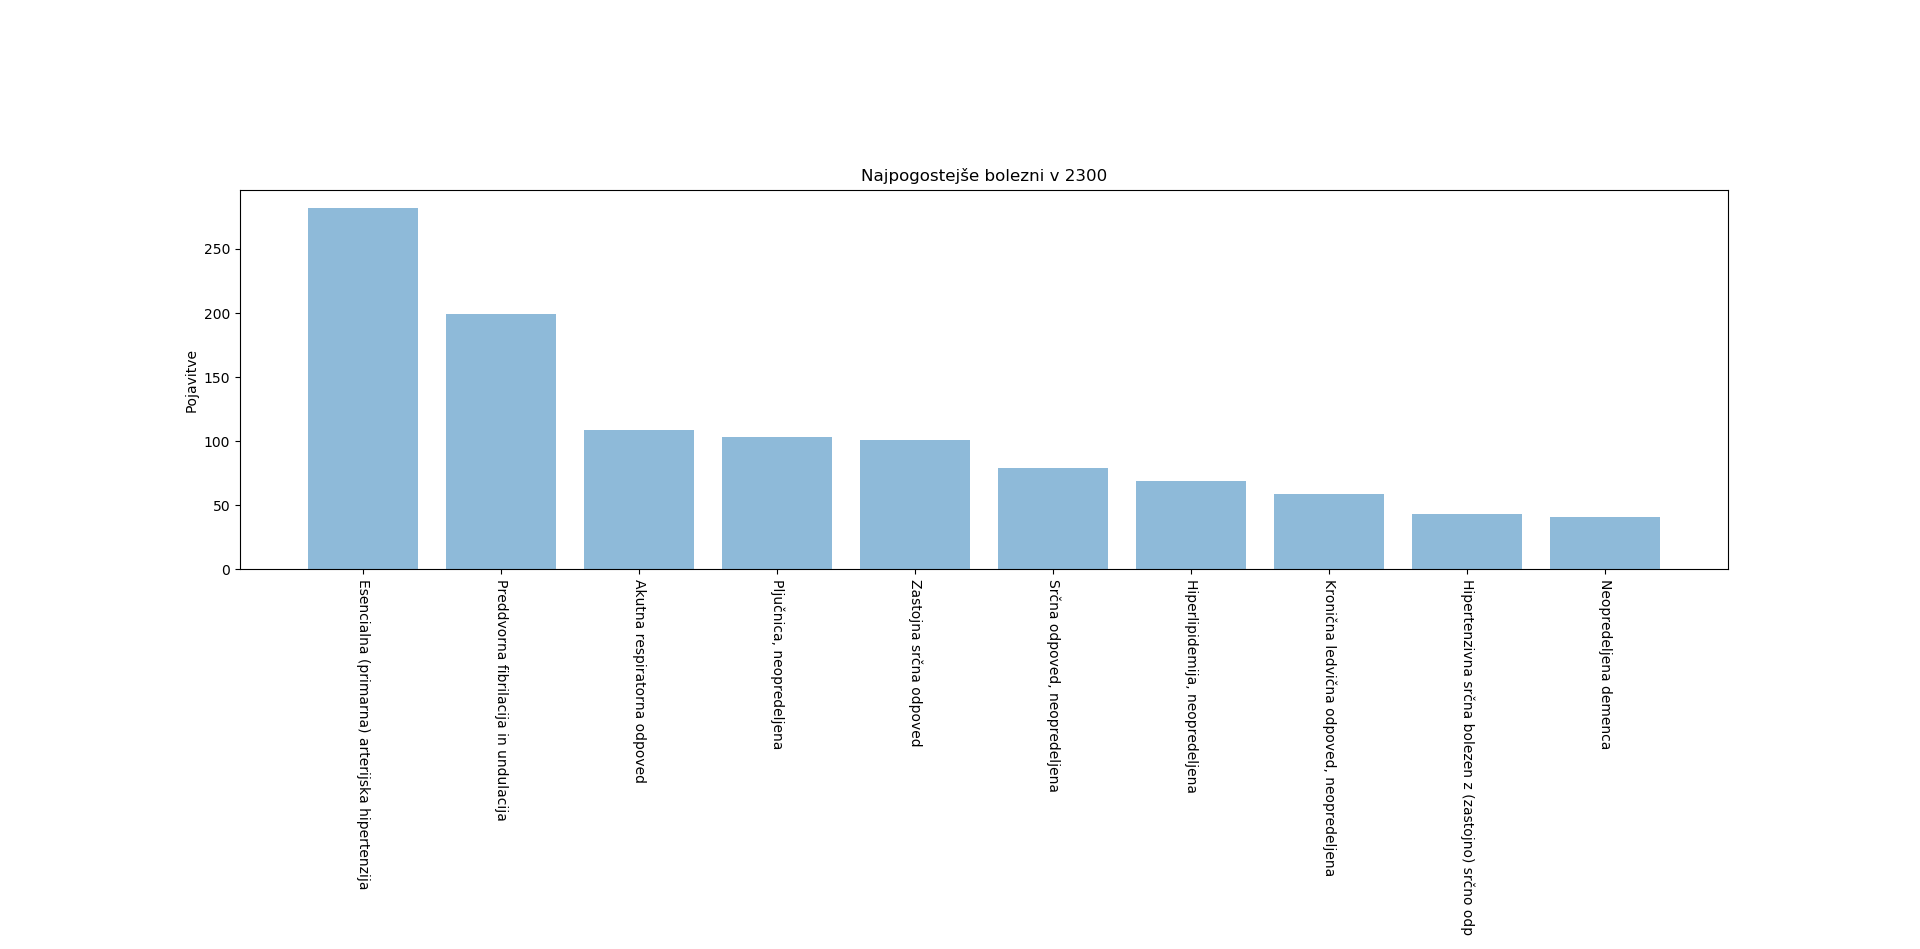
\includegraphics[width=\linewidth]{./grafi/2300.png}
            \caption{Najpogostejše bolezni - oddelek 2300}
         \end{minipage}
         \hfill
         \begin{minipage}[b]{0.4\textwidth}
            \noindent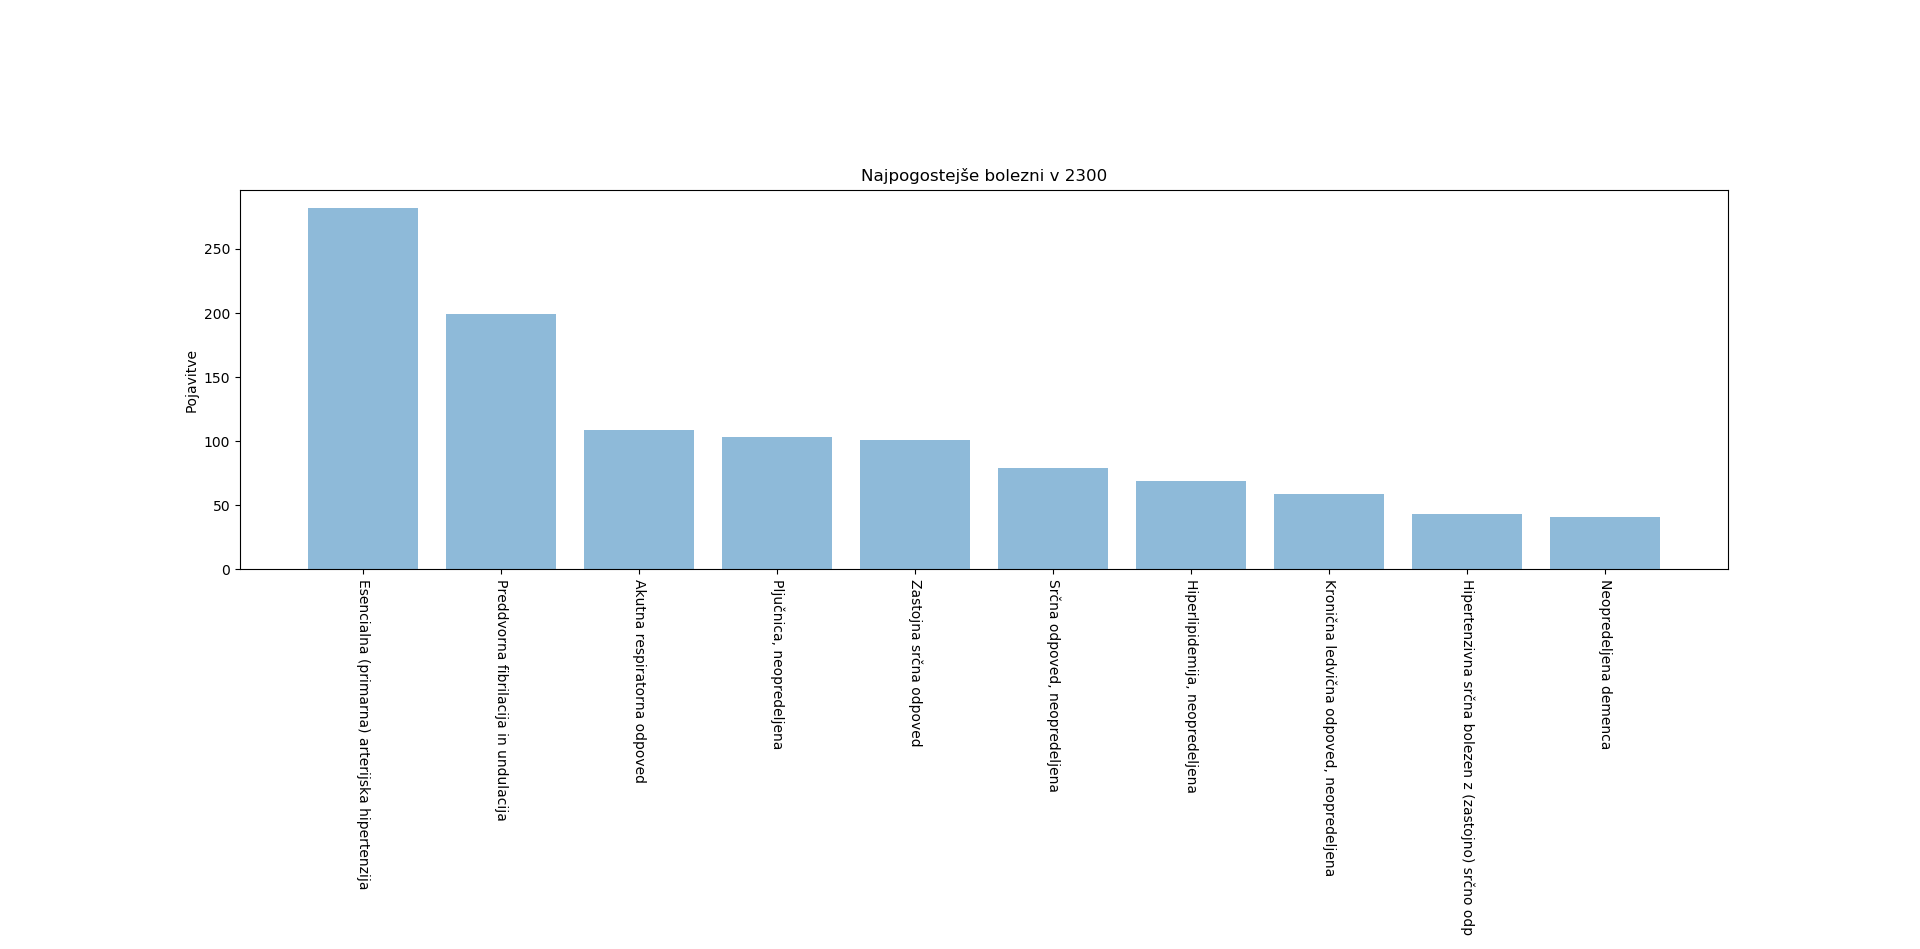
\includegraphics[width=\linewidth]{./grafi/2300.png}
            \caption{Najpogostejše bolezni - oddelek 2301}
         \end{minipage}
   \end{figure}

   \begin{figure}[!htb]
      \centering
         \begin{minipage}[b]{0.4\textwidth}
            \noindent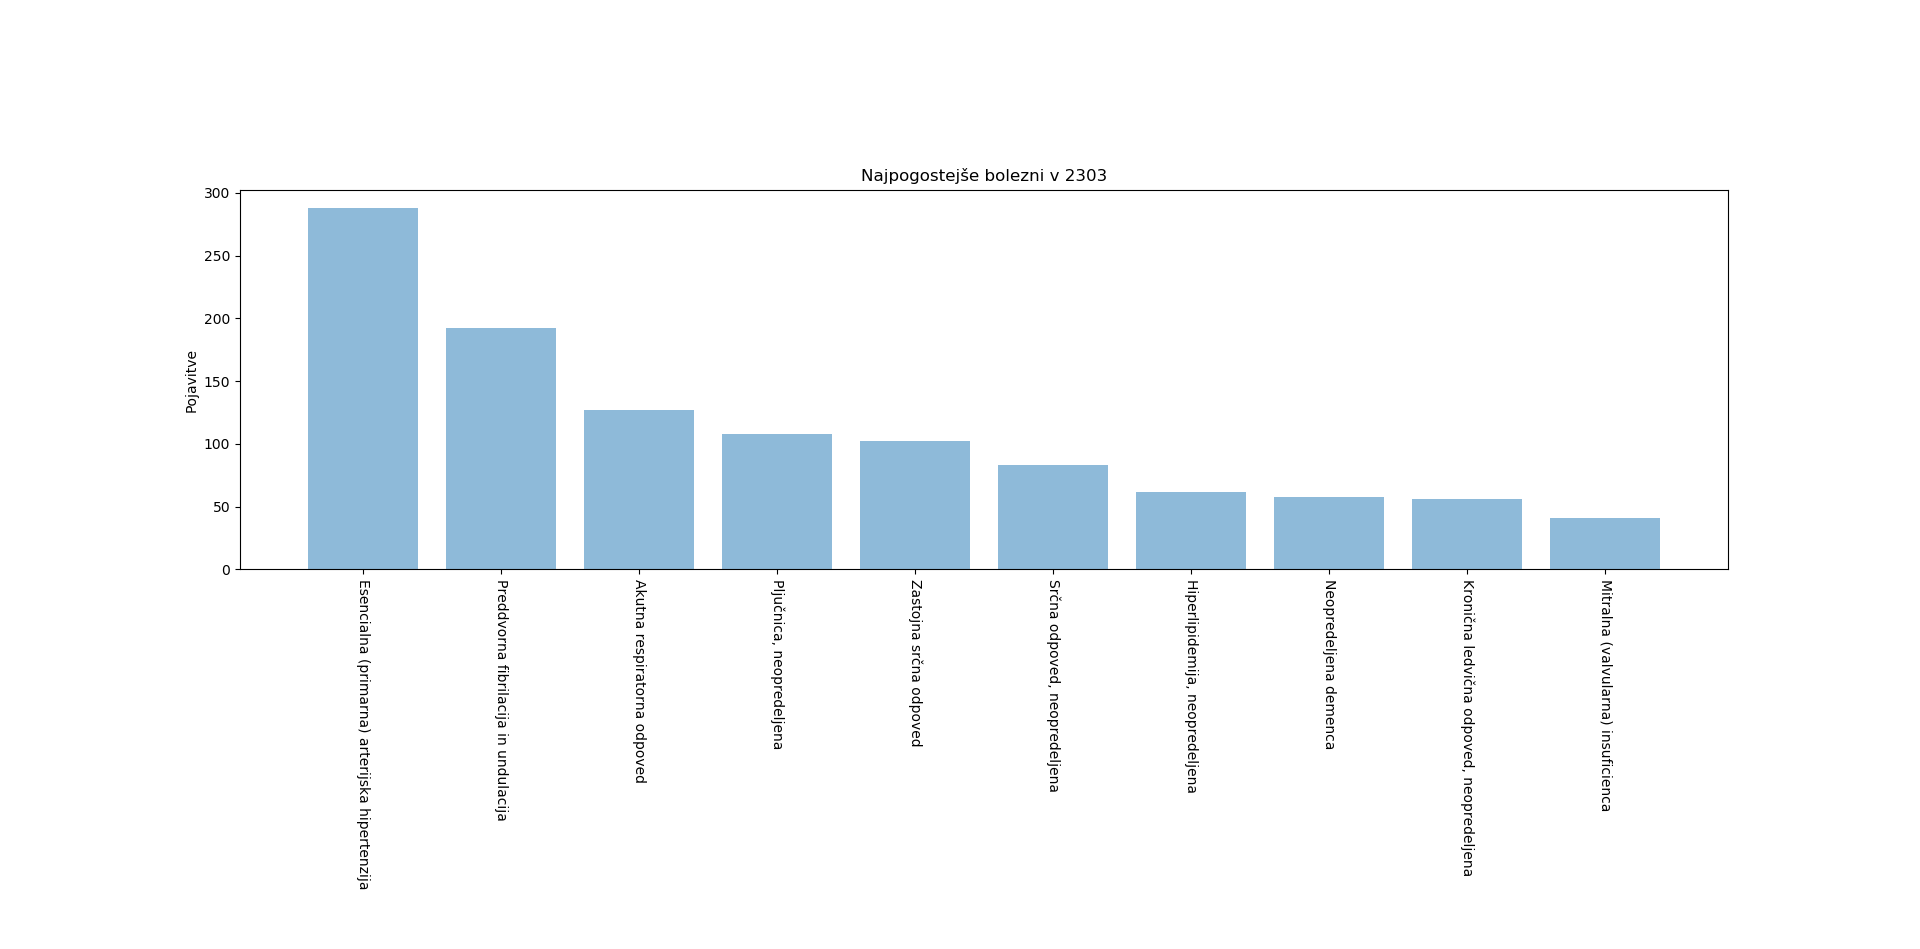
\includegraphics[width=\linewidth]{./grafi/2303.png}
            \caption{Najpogostejše bolezni - oddelek 2303}
         \end{minipage}
         \hfill
         \begin{minipage}[b]{0.4\textwidth}
            \noindent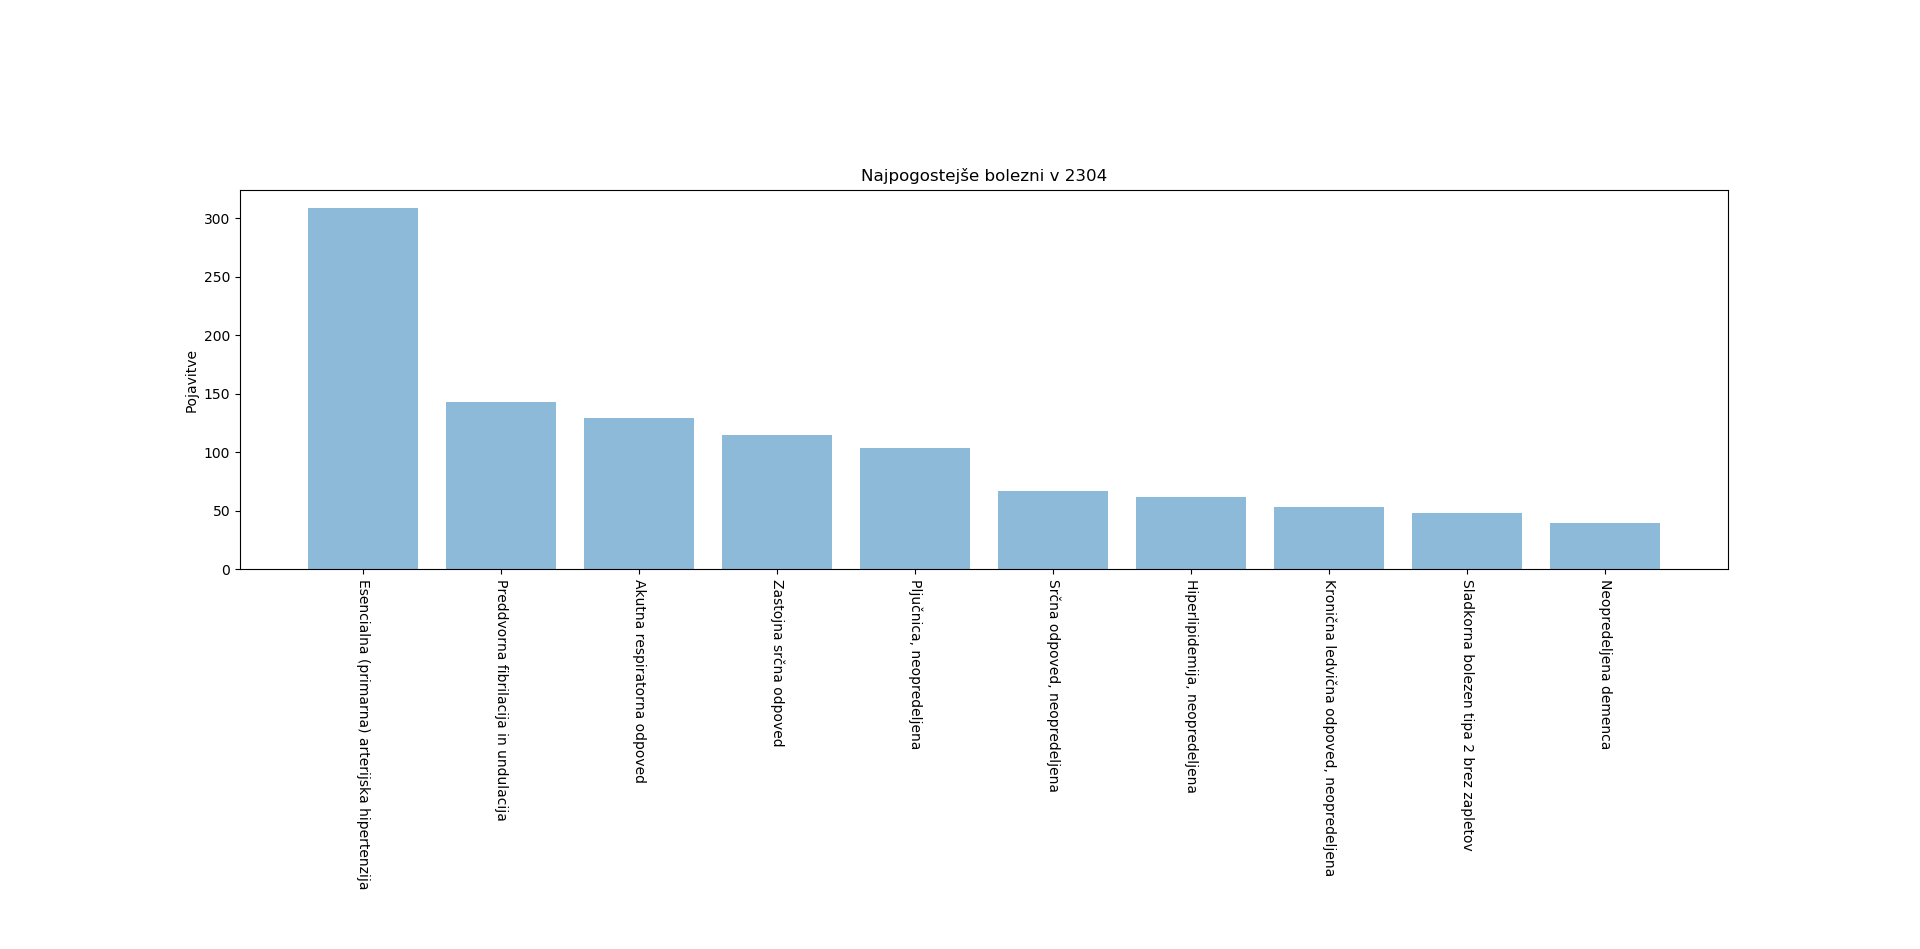
\includegraphics[width=\linewidth]{./grafi/2304.png}
            \caption{Najpogostejše bolezni - oddelek 2304}
         \end{minipage}
   \end{figure}

   \begin{figure}[!htb]
      \centering
         \begin{minipage}[b]{0.4\textwidth}
            \noindent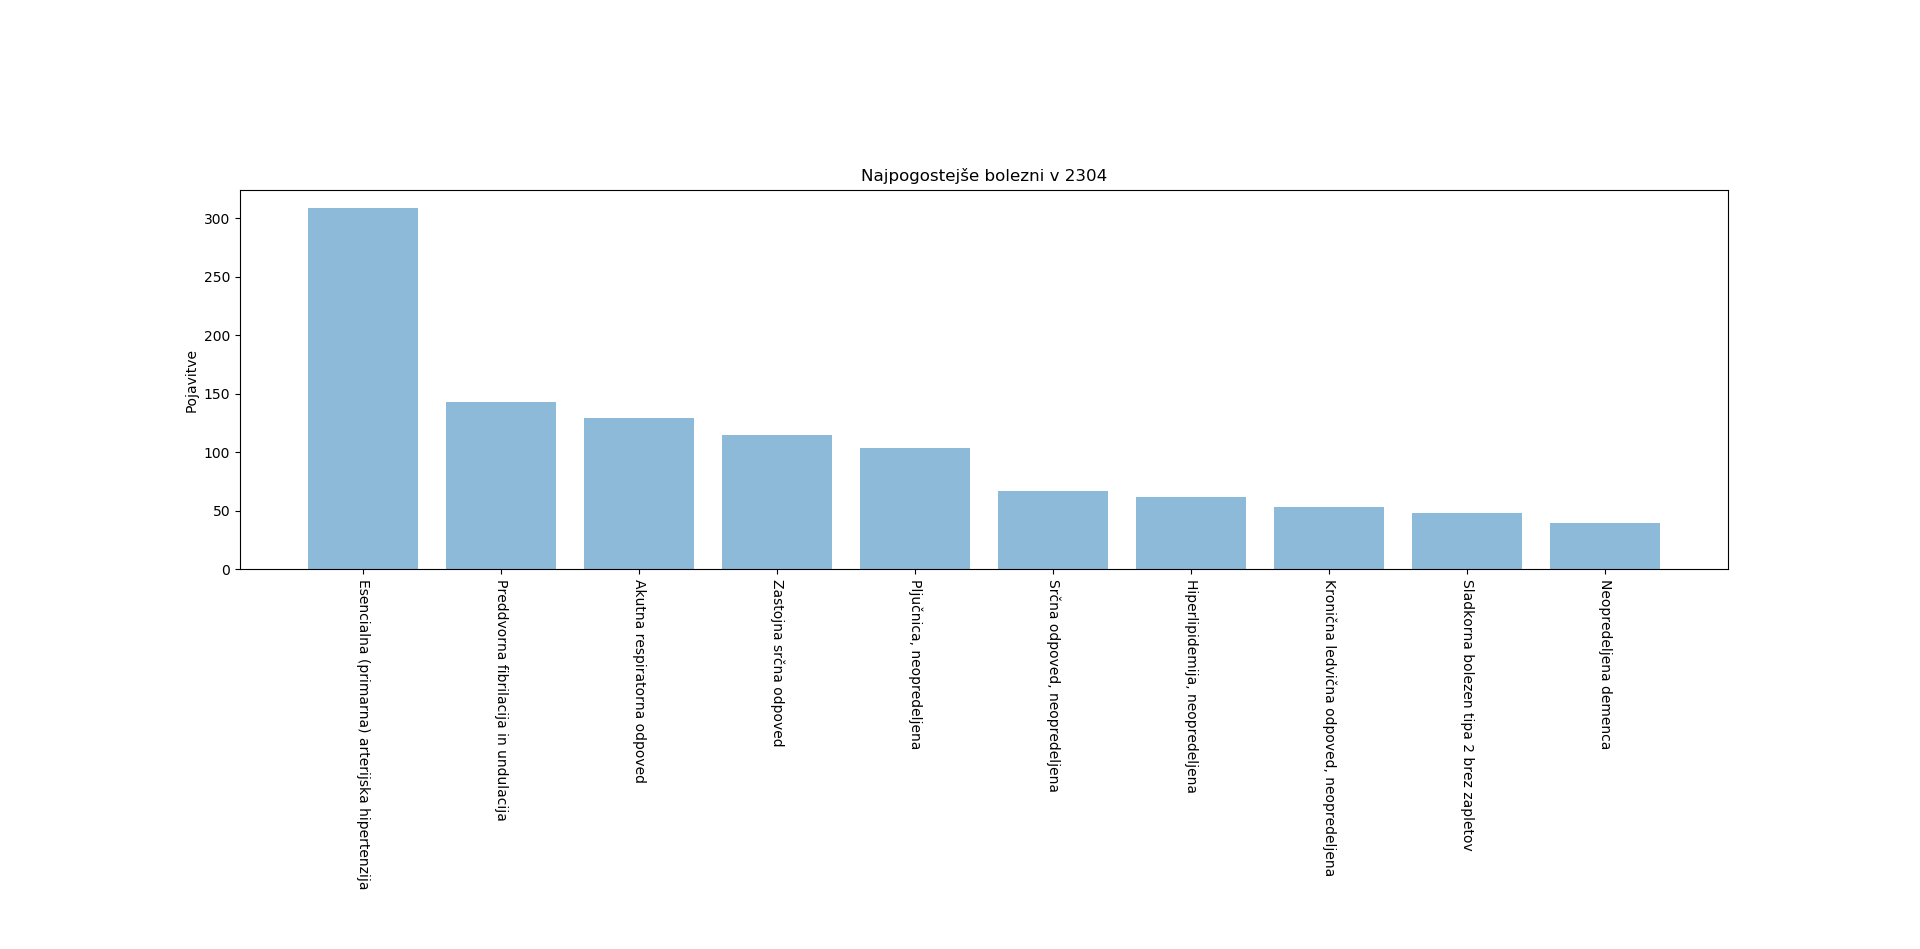
\includegraphics[width=\linewidth]{./grafi/2304.png}
            \caption{Najpogostejše bolezni - oddelek 2305}
         \end{minipage}
         \hfill
         \begin{minipage}[b]{0.4\textwidth}
            \noindent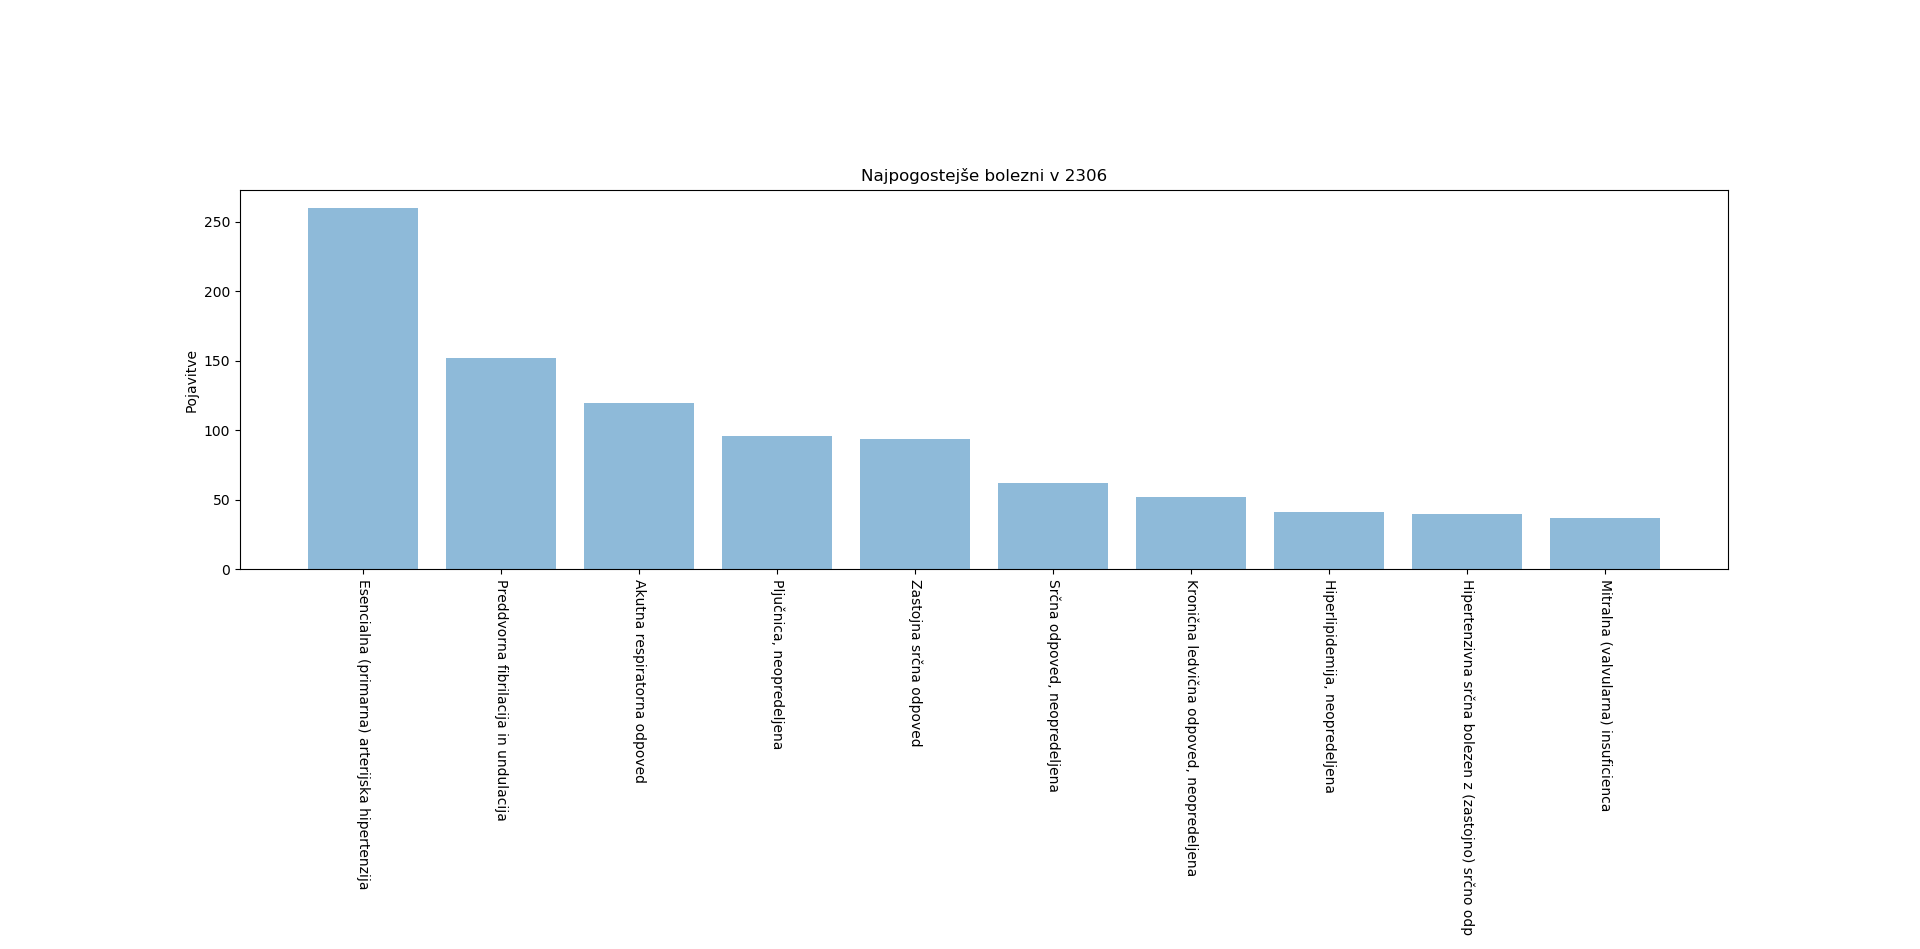
\includegraphics[width=\linewidth]{./grafi/2306.png}
            \caption{Najpogostejše bolezni - oddelek 2306}
         \end{minipage}
   \end{figure}

   \begin{figure}[!htb]
      \centering
         \begin{minipage}[b]{0.4\textwidth}
            \noindent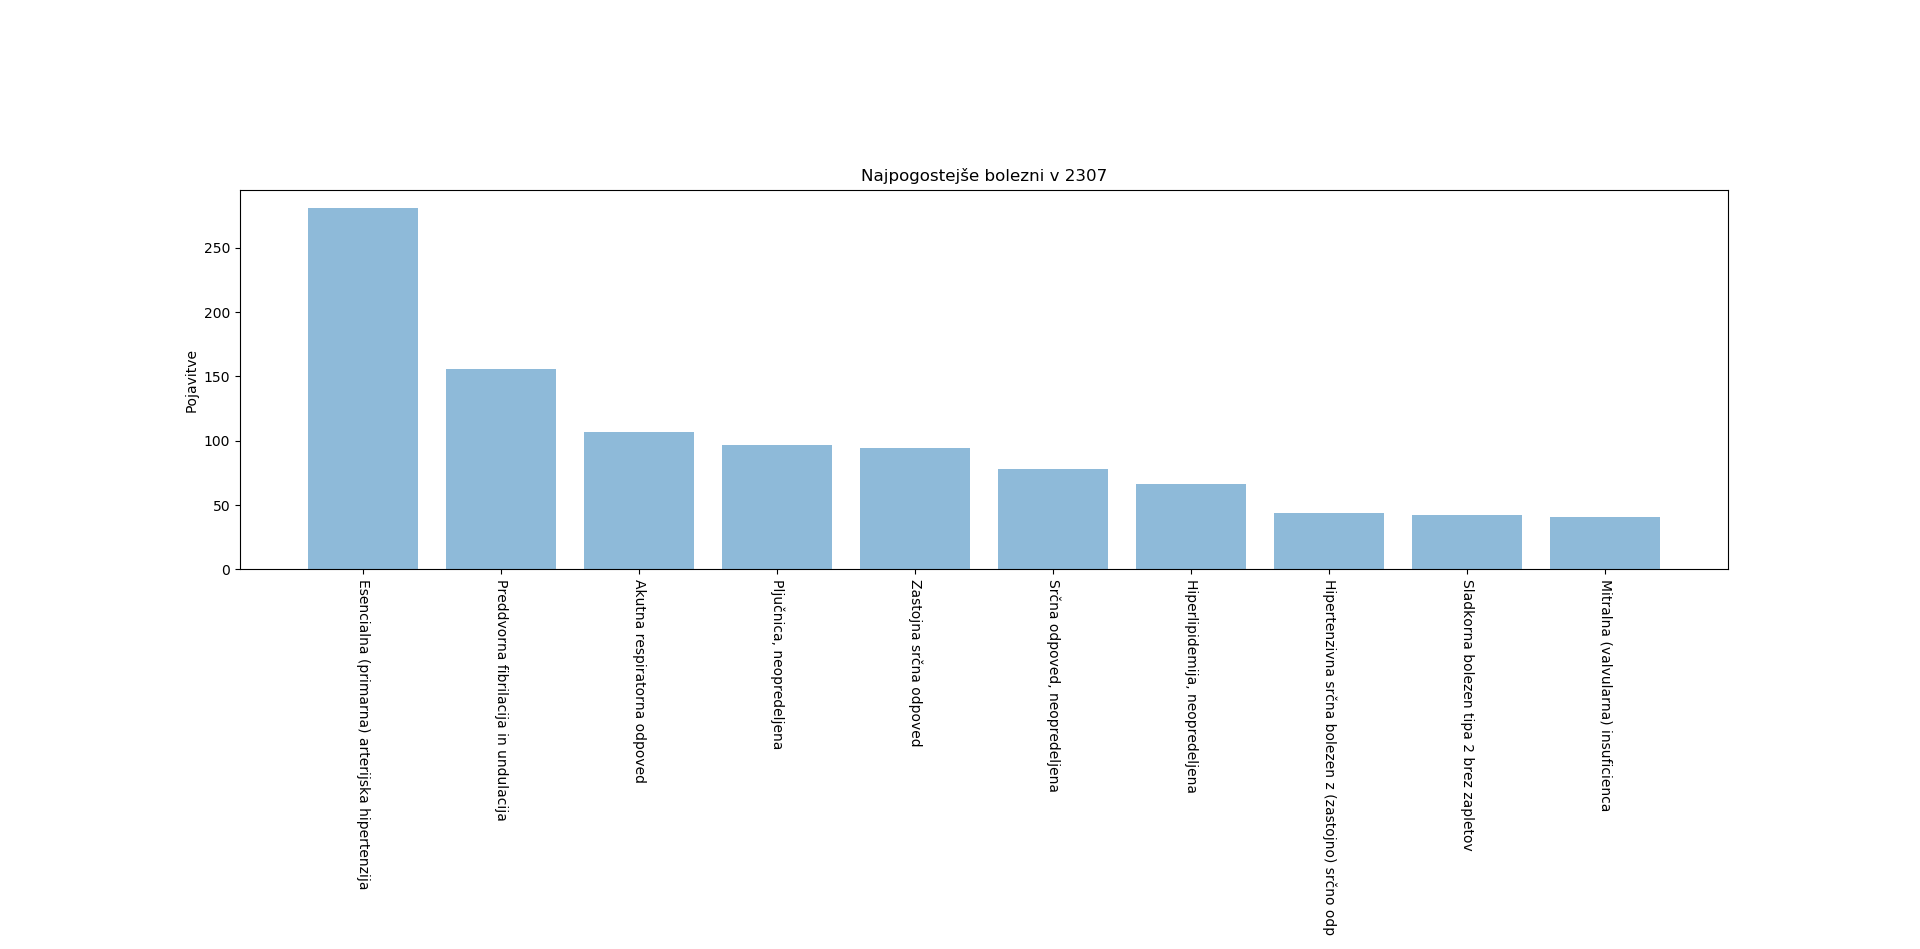
\includegraphics[width=\linewidth]{./grafi/2307.png}
            \caption{Najpogostejše bolezni - oddelek 2307}
         \end{minipage}
         \hfill
         \begin{minipage}[b]{0.4\textwidth}
            \noindent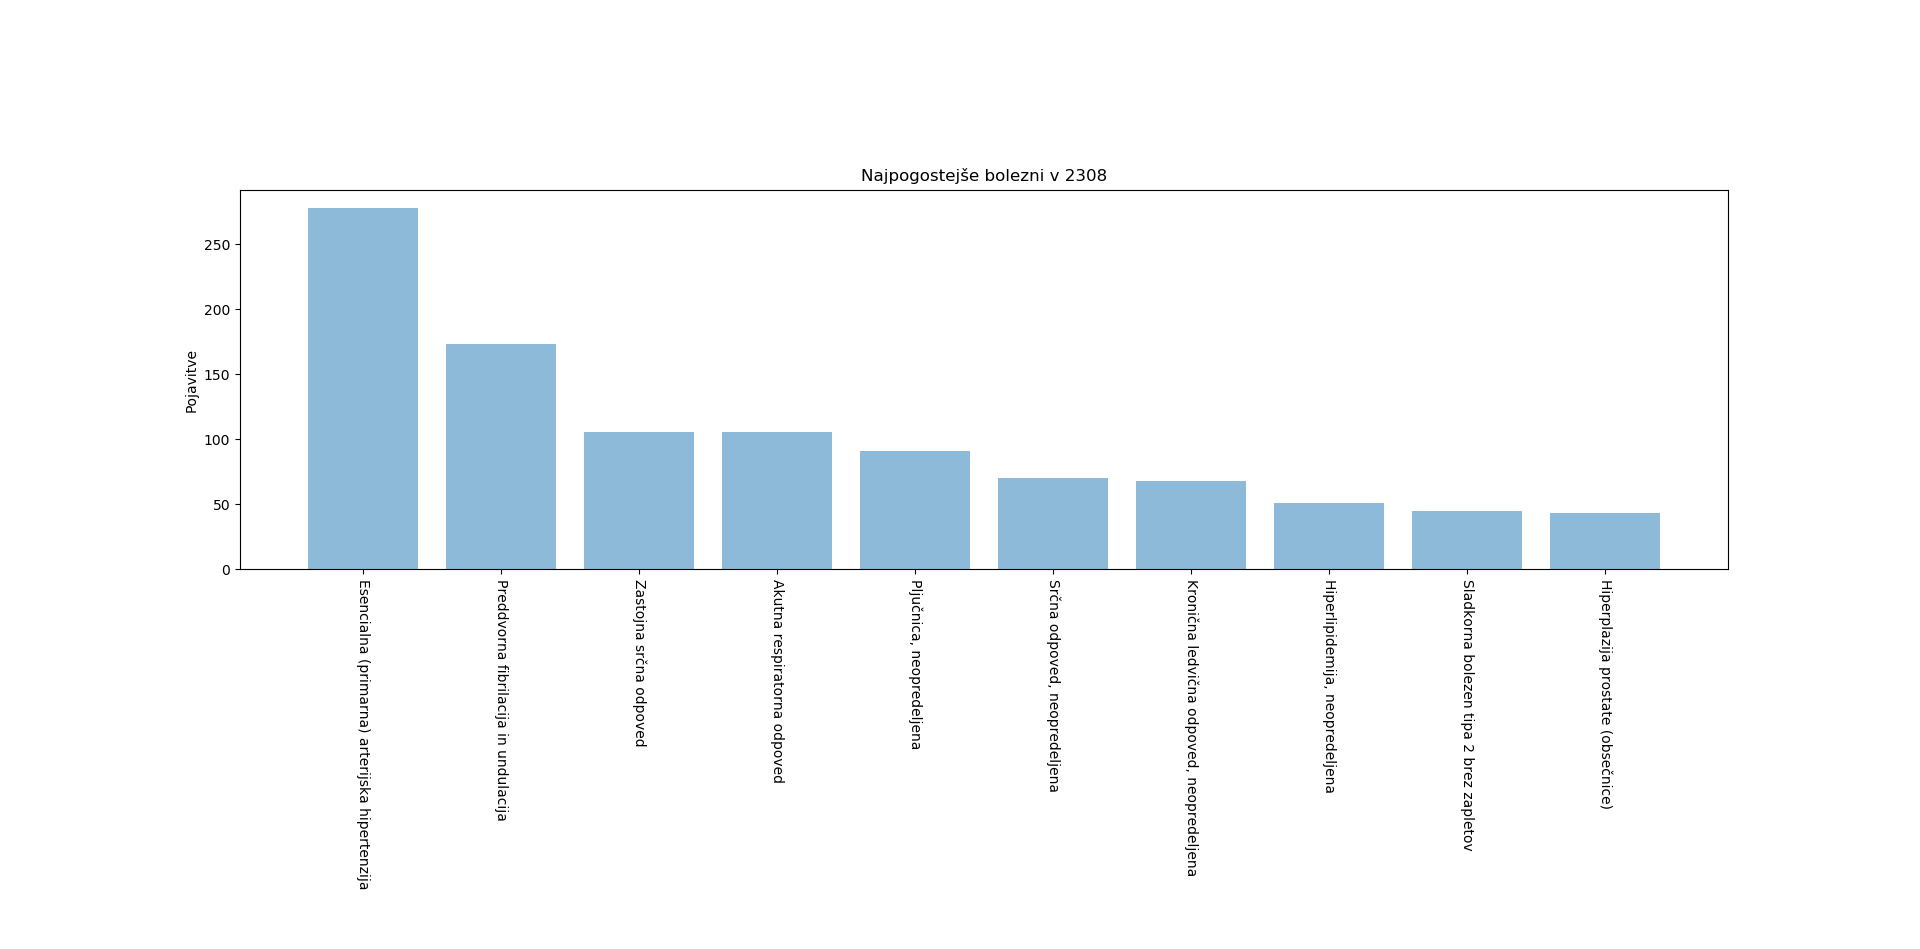
\includegraphics[width=\linewidth]{./grafi/2308.png}
            \caption{Najpogostejše bolezni - oddelek 2308}
         \end{minipage}
   \end{figure}

   \begin{figure}[!htb]
      \centering
         \begin{minipage}[b]{0.4\textwidth}
            \noindent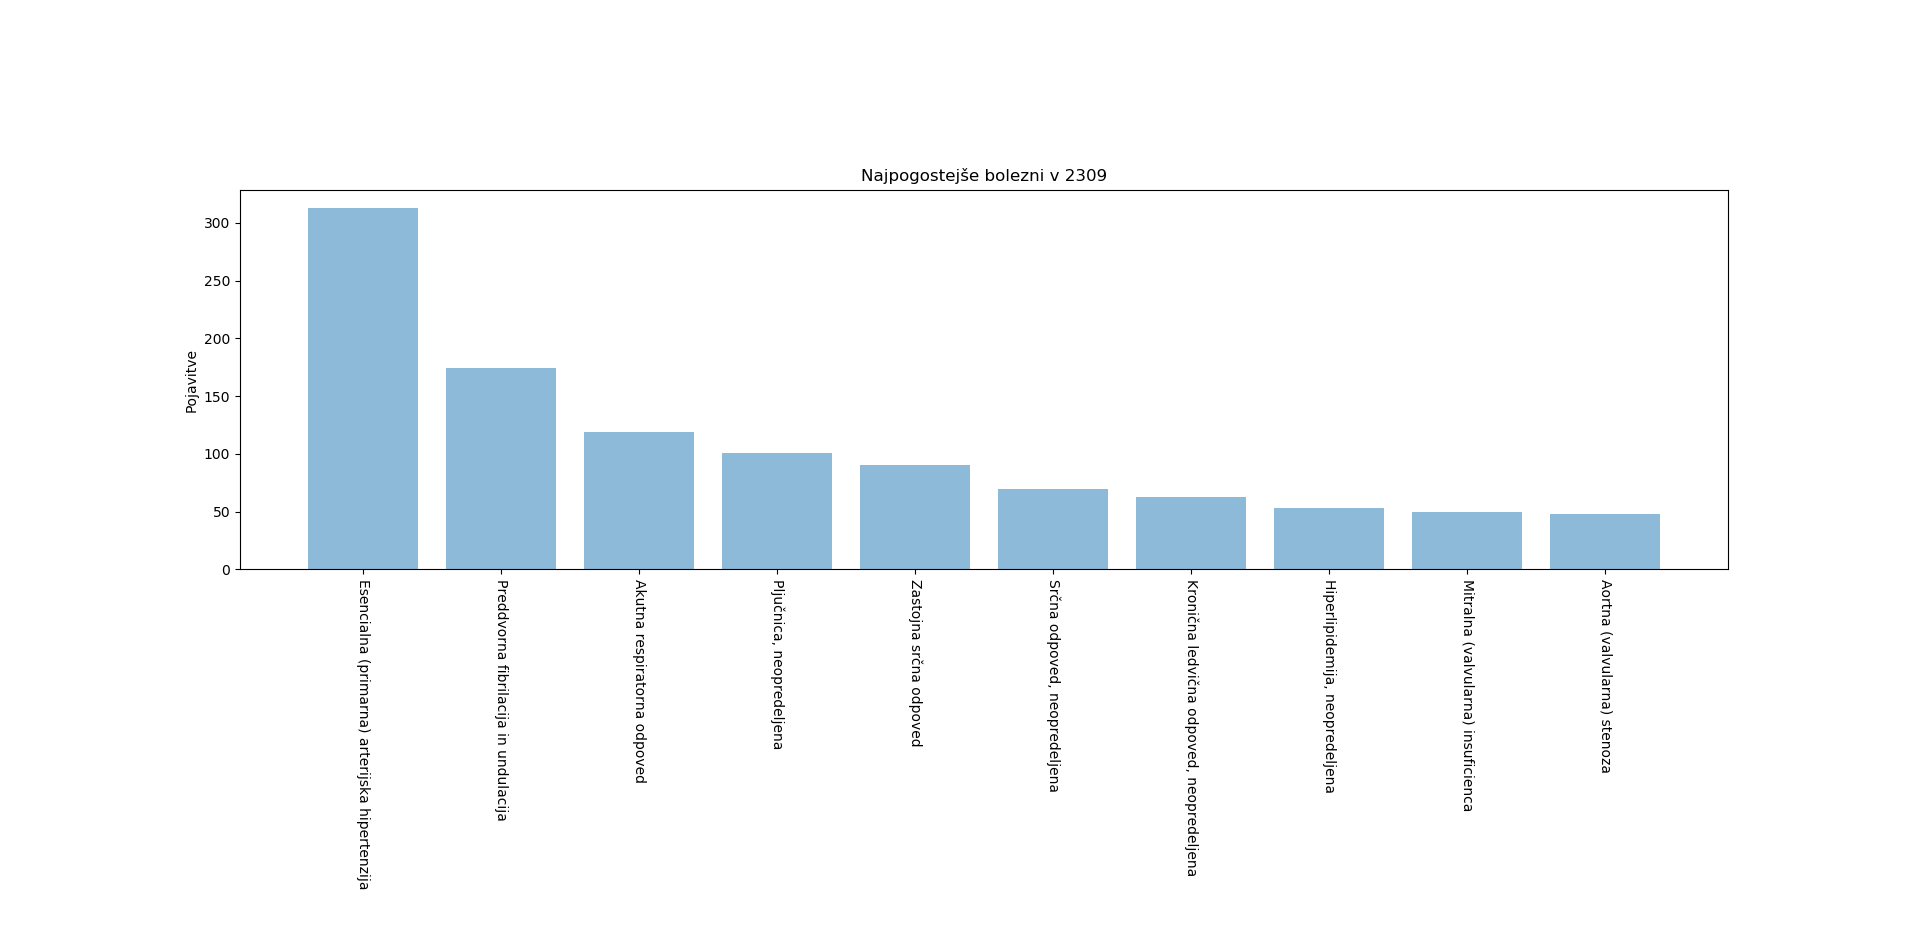
\includegraphics[width=\linewidth]{./grafi/2309.png}
            \caption{Najpogostejše bolezni - oddelek 2309}
         \end{minipage}
         \hfill
   \end{figure}

   \begin{figure}[!htb]
      \centering
         \begin{minipage}[b]{0.4\textwidth}
            \noindent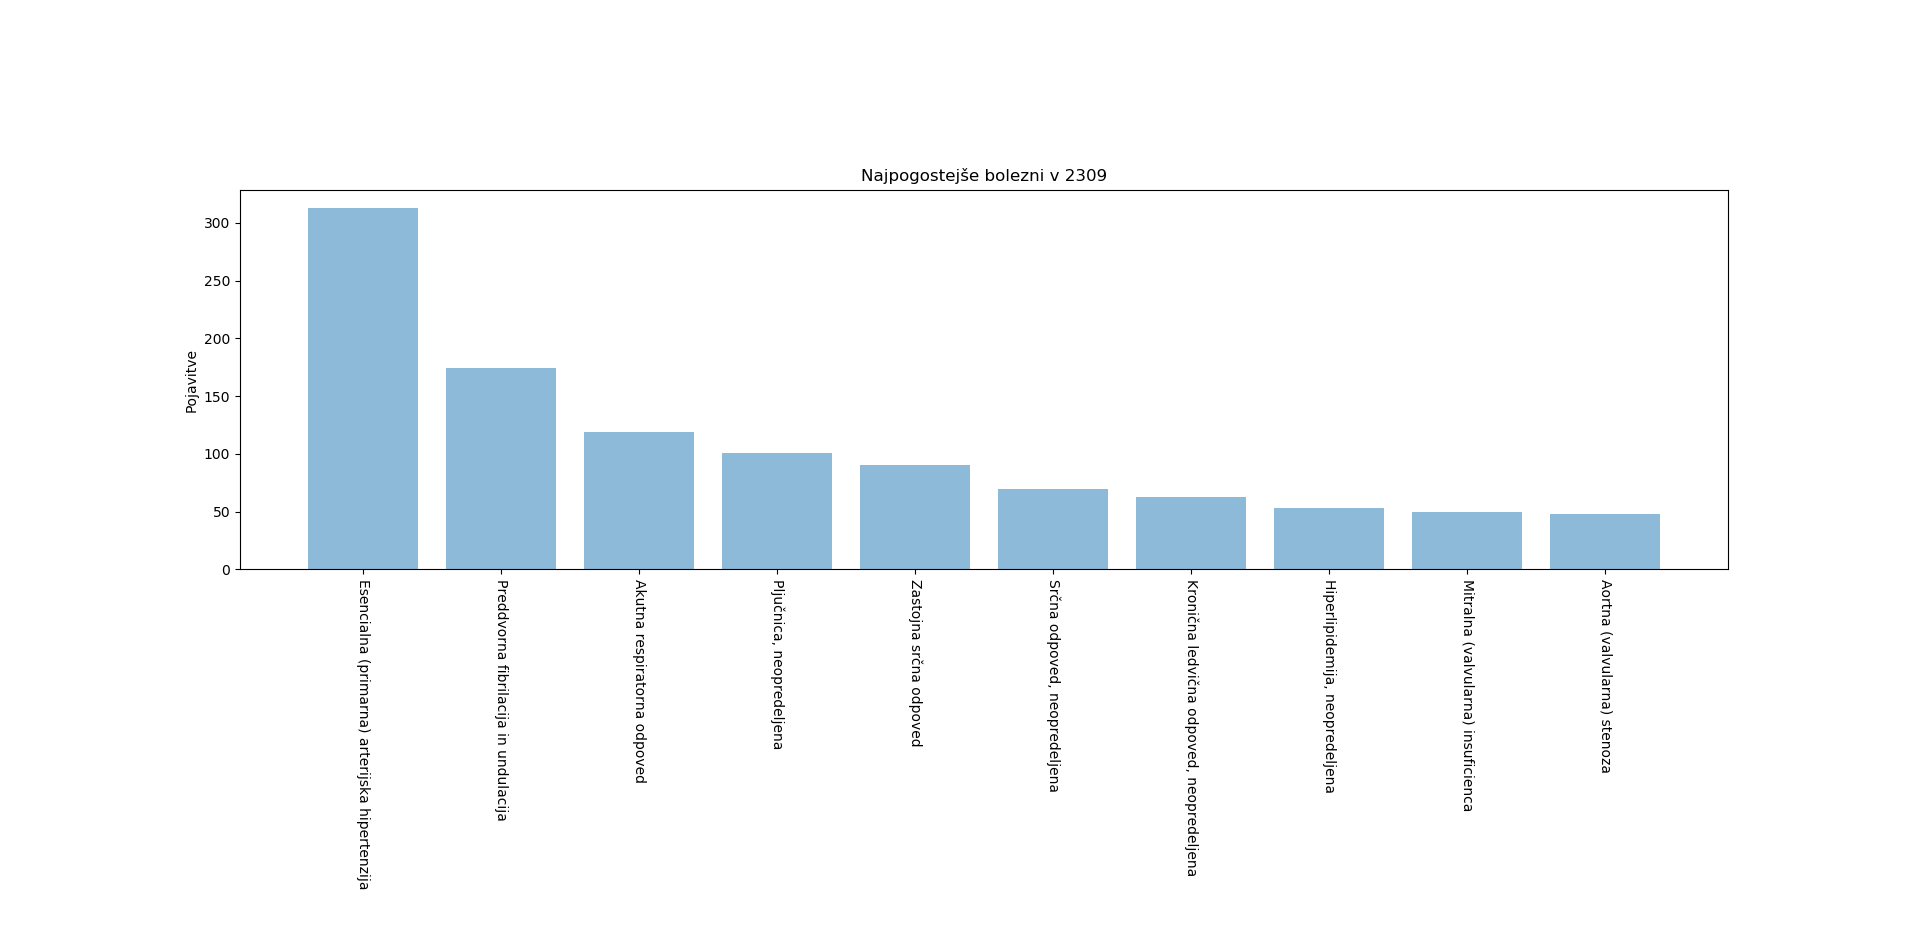
\includegraphics[width=\linewidth]{./grafi/2309.png}
            \caption{Najpogostejše bolezni - oddelek 2309}
         \end{minipage}
         \hfill
         \begin{minipage}[b]{0.4\textwidth}
            \noindent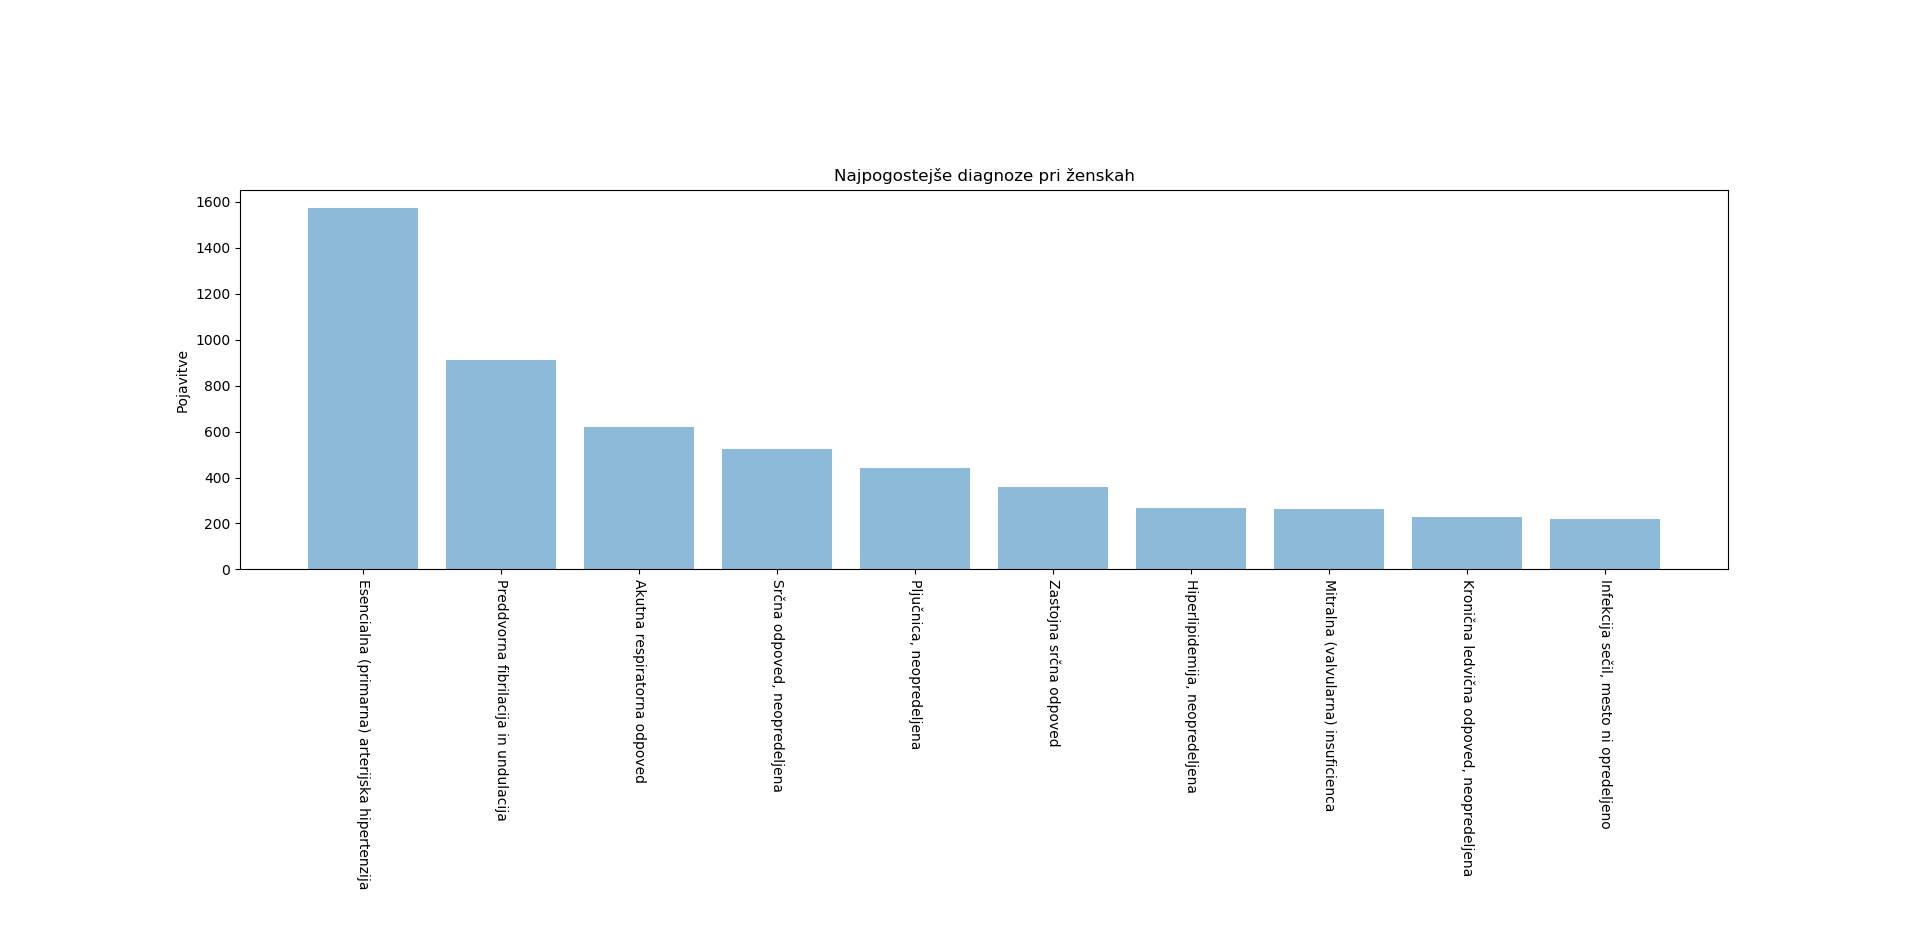
\includegraphics[width=\linewidth]{./grafi/zenske.png}
            \caption{Najpogostejše bolezni - ženske}
         \end{minipage}
   \end{figure}

\end{center}

\section*{Naloga (d)}
\paragraph{Navodila}
Ugotovite razliko med MKB kodami in WHO ICD kodami (katere so tiste, ki jih drugi ne pozna), ter jih predstavite v Excelovi tabeli urejene glede na število pojavitev med diagnozami.

\pagebreak
\paragraph{Kode, ki so del WHO, niso del MKB}
Tabela prikazuje kode, ki so del nabora kod WHO, vendar niso nabor kod MKB. \textit{Kode, ki med diagnozami nimajo vnosa niso navedene}:

\begin{center}
   \begin{tabular}{||c|r||}
      \hline
      WHO koda & Število diagnoz\\
      \hline
      \hline
      N18.8 & 59\\
      N18.0 & 20\\
      T28.6 & 10\\
      T28.7 & 7\\
      R73.9 & 4\\
      R50.0 & 4\\
      T28.5 & 3\\
      U80.1 & 2\\
      N08.3 & 2\\
      R73.0 & 1\\
      E90 & 1\\
      J99.0 & 1\\
      H36.0 & 1\\
      H82 & 1\\
      G63.2 & 1\\
      \hline

   \end{tabular}
\end{center}

\pagebreak
\paragraph{Kode, ki so del MKB, niso del WHO}
Tabela prikazuje 20 najpogostejših kod, ki se pojavljajo med diagnozami, ki so del nabora kod MKB, vendar niso nabor kod WHO. 
Vseh kod, ki so del nabora MKB, vendar ne WHO, je 1146.\textit{Kode, ki med diagnozami nimajo vnosa niso navedene}:

\begin{center}
   \begin{tabular}{||c|r||}
      \hline
      MKB koda & Število diagnoz\\
      \hline
      \hline
      I48 & 1739\\
      J96.0 & 1148\\
      I50.0 & 972\\
      F03 & 383\\
      N40 & 287\\
      X61 & 230\\
      I69.4 & 224\\
      E11.7 & 208\\
      Z98.8 & 182\\
      T42.4 & 180\\
      J45.9 & 174\\
      E14.9 & 151\\
      T58 & 141\\
      I69.3 & 135\\
      J96.9 & 134\\
      I25.1 & 132\\
      I25.0 & 132\\
      K70.3 & 130\\
      E11.71 & 120\\
      Z92.1 & 106\\
      \hline

   \end{tabular}
\end{center}

\end{document}